\documentclass[a4paper,12pt]{article} % Prepara un documento per carta A4, con un bel font grande
 
\usepackage[italian]{babel} % Adatta LaTeX alle convenzioni tipografiche italiane,
% e ridefinisce alcuni titoli in italiano, come "Capitolo" al posto di "Chapter", se il vostro documento è in italiano
\usepackage[T1]{fontenc} % Riga da togliere se si compila con PDFLaTeX
\usepackage[utf8]{inputenc} % Consente l'uso caratteri accentati italiani
\usepackage{listings}
\lstset{language=C}
 \usepackage{graphicx}
\frenchspacing % forza LaTeX ad una spaziatura fra parole non inglesi
 
\title{Appunti di Linux} % \LaTeX è una macro che compone il logo "LaTeX"
% I commenti (introdotti da %) vengono ignorati
\begin{document}
\maketitle % Produce il titolo a partire dai comandi \title, \author e \date
\tableofcontents % Prepara l'indice generale

\section{Comandi utili}
\begin{itemize}
\item  \textit{ls} Mostra la lista dei file e delle cartelle nella directory corrente
\item  \textit{ls -l} Mostra una lista più dettagliata
\item  \textit{touch} nomefile : crea un nuovo file chiamato nomefile
\item  \textit{ls >}z Mette l'outuput del comando dentro un nuovo file z
\item  \textit{ls <}z Prende l'input del comando da un file z
\item  \textit{cut -f 1 -d ' '} Taglia il primo campo (field -f 1) rispetto al delimitatore ' '
%\item  \textit{}
\end{itemize}

\section{I filtri di Unix}
Unix mette a disposizione tanti filtri utili (molti saranno discussi dopo) da usare con la tecnica del pipelining. Eccone alcuni:
\begin{itemize}
\item \textit{sort} Ordina un qualsiasi flusso in input (sia esso un file o l'output di less)
\item \textit{grep,awk} Discussi in seguito.
\item \textit{uniq} Filtra le linee ripetute in un file.
\end{itemize}

\section{I Processi in Linux} 
Ogni processo in Linux nasce con tre canali: stdin, stdout ed stderr.
Il primo serve per gestire gli input da tastiera, i secondi due per l'output e gli errori, che sono visualizzati presso il monitor del TTY corrente.
Per ogni processo che è in esecuzione in Linux posso inviare dei \textit{signals} quali:
\begin{itemize}
\item STOP: Voglio fermare il mio processo. \textit{CTRL + Z}
\item TERM: Voglio terminare il mio processo. \textit{CTRL + C}
\end{itemize}
\subsection{Processi in background,foreground o attivi}
Bene, abbiamo visto come interrompere o terminare un processo. Ma se vogliamo fare il resume dell' ultimo processo fermato?
Basta scrivere \textit{fg} che sta per foreground (in sovraimpressione).
Se invece voglio resumare quel processo ma voglio che sia fatto in background allora basta digitare \textit{bg \% id-processo}.
Se invece voglio lanciare un processo direttamente in background senza passare per il bg basta invocarlo con l'opzione \textit{\&}
Altro comando utile è \textit{jobs} che fornisce la lista di tutti i job su quel tty.
\subsection{La lista dei processi}
I processi attivi sul calcolatore si posso mostrare con il comando \textit{ps aux} alias di processes, mostra tutti i processi attivi.
Se nel campo STAT c'è la S vuol dire che quel processo è in Sleeping, mentre se c'è la R vuol dire che è in running.
\textit{Tips:} Per leggere più comodamente mando l'output a less col comando pipe: \textit{ps -lax | less} dove quel -lax mi da una versione più dettagliata.
Altre varianti:
\begin{description}
\item \textit{pstree} mostra i processi con struttura ad albero.
\item \textit{pstree -p} mostra i processi con struttura ad albero compresi i pid di ogni processo.
\end{description}
\subsubsection{Uccidere i processi}
Si hanno due possibilità:
\begin{itemize}
\item \textit{kill} pid uccide il processo con quel pid.
\item \textit{kill -9} uccide il processo in modo perentorio.
\end{itemize}

\subsection{La tecnica del pipelining}
E' una tecnica molto ultile che permette di attaccare il file stdout di un processo al file stdin di un altro creando curiose catene
Esempio:
\begin{description}
\item \textit{ls} | \textit{tr l z} Invoca la lista, prende l'output e lo manipola. In che modo? Sostituendo (tr) le lettere l con z.
\item \textit{ls} | \textit{head -n} Mostra i primi n file di una directory. Senza niente mostra i primi 10 file.
\item \textit{ls} | \textit{tail -n} Mostra gli ultimi n file di una directory. Senza niente mostra gli ultimi 10 file.
\item \textit{ls} | \textit{wc} Conta le frasi,parole e caratteri.
\end{description}

\subsection{Un primo approccio pratico: Manipoliamo passwd}
\emph{Obiettivo: Sapere quante occorrenze della stringa /usr/bin/false ci sono nel file.} \\ \\
Abbiamo già parlato di passwd dicendo che curiosamente non contiene le password di sistema ma una serie di record con campi che servono al sistema per gestire utenti e demoni. Essendo la sua struttura così ben predisposta
alla manipolazione andremo ad eseguire operazioni sull' output dello stesso.
\begin{itemize}
\item \textit{Fase 1: Modifichiamo il separatore:} andiamo a modificare il separatore dei campi in passwd: \\ cat /etc/passwd | tr : ""$\backslash$n"" | less
\item \textit{Fase 2: Ordinare i campi:} per far ciò usiamo l'ottimo filtro \textit{sort}: \\ cat /etc/passwd | tr : ""$\backslash$n"" | sort | less
\item \textit{Fase 3: Eliminare i doppioni:} per far ciò utilizziamo \textit{uniq} che si applica ad un output già ordinato: \\ cat  cat /etc/passwd | tr : ""$\backslash$n"" | sort | uniq -c | less . \\ Con l'opzione -c accanto al nome vedo anche
								quante volte compare il campo (era ciò che volevamo)
\item \textit{Fase 4: Ordinare in ordine numerico anzichè alfabetico e mostrare la classifica:} per far ciò usiamo \textit{sort -nr} che ordina in modo inverso e numerico e \textit{head} che ci mostra i primi 10: \\ 
																	      cat  /etc/passwd | tr : ''$\backslash$n'' | sort | uniq -c | sort -nr | head															      	
\end{itemize}
\section{I filtri Grep e Awk}
\begin{description}
\item \textit{Grep:} permette di effettuare selezione di righe in output secondo pattern matching (espressioni regolari)
\item \textit{Awk:} permette di fare le stesse cose di grep, ma è più potente perchè è un vero e proprio linguaggio di programmazione.
\subsection{Grep}
\subsubsection{Le espressioni regolari}
Una espressione regolare è a tutti gli effetti un pattern: \\
Es.\\
\begin{itemize}
\item \textit{grep 'a'}: riporta tutti gli output contenenti a
\item \textit{grep 'ab?c'}: ? si applica all'oggetto prima e specifica che quell' oggetto può esserci o non esserci
 \item \textit{grep 'ab*c'}: * si applica all'oggetto prima e specifica che quell' oggetto deve esserci almeno una volta o n volte
 \item \textit{grep -E '(a | b)'}: matcha a o b. Per usare la pipe | e le parentesi ( )  si deve avviare grep con l'opzione -E 
 \item \textit{grep -v espressione\_regolare}: toglie i risultati matchati dall' output
 \item \textit{grep '[a-z]'}: è equivalente a: a|b|c|....z
 \item \textit{grep '[0-9]'}: è equivalente a 0|1|...9
 \item \textit{. }: Il punto rappresenta un carattere qualsiasi.
\end{itemize}
Esempi:\\
\begin{description}
\item \textit{grep ' \^""[0-9]*\$'} : Matcha una parola fatta solo di cifre. \^"" è  il delimitatore di inizio riga, \$ è il delimitatore di fine riga.
\item \textit{grep -v '\^""\$'} : Toglie tutte le righe vuote.
\item \textit{$\backslash$}: Serve a matchare caratteri speciali.
\end{description}

\subsubsection{Esempi pratici su /etc/passwd}
Alcuni esempi di matching:\\
\textit{cat /etc/passwd | grep ':/var[\^"":]*:'} : matcha un qualsiasi campo con dentro var. Notare come [\^"":] significhi "qualsiasi carattere tranne i due punti".\\
\textit{cat /etc/passwd | grep ':[\^"":]*\$'} : matcha l'ultimo campo.\\
Uniamo i due risultati: \\
\textit{cat /etc/passwd | grep ':/var[\^"":]*:[\^"":]*\$'}: matcha il penultimo campo contenente var
\end{description}

\subsection{Awk}
Ha una sintassi del tipo:\\
\begin{center}
awk '[BEGIN\{\}] /pattern/ \{action\} [END\{\}]'
\end{center}
BEGIN e/o AND sono opzionali.
All' interno di pattern o action posso usare delle variabili:\\
\$0 : L'intera riga.\\
\$1: Il primo campo.\\
\$N : l'N-esimo campo.
I campi sono delimitati di default da spazi e tabulatori, per cambiare il delimitatore di campo:
\begin{center}
[...]BEGIN\{FS= '':'' \}[...il resto del programma...]\\
oppure:\\
awk -v FS=: [...il resto del programma...]
\end{center}
\subsubsection{Awk e le stringhe}
L'unico tipo di dato che esiste in awk è il tipo stringa. Anche operazioni come somme o sottrazioni possono essere fatte ma restituiscono stringhe.
Ci sono alcune variabili paraticolari in awk:\\
\textit{NF}: Number of Fields\\
\textit{NR}: Number of Records\\
\textit{OFS}: Output Field Separator\\
\subsubsection{Alcuni Esempi}
\textit{awk '\$1 \~""/pippo/'} : (tilde è il carattere ascii) Matcha \$1 con pippo\\
\textit{awk '/pippo/ \{s = s+1\} END\{print s\}}': Stampa le occorrenze di pippo\\
\textit{awk 'for(i=1;i<=NF;i++) print i'}: Stampa il numero incrementale dei campi.\\
\textit{awk '\{print \$NF \}'}: il valore dell' ultimo campo (NF stampa il numero dell' ultimo campo)\\
\textit{awk '\{print \$(NF-1) \}'}: il valore del penultimo campo.\\
\textit{awk '\{if (\$7 == ''/bin/sh/'') print \$1,\$7\}'}: Stampa tutte le occorrenze di \$7 associate al primo campo. La virgola introduce un field separator tra i due campi.
\textit{awk '\{print \$2,\$1 \}'}: Ribalta due campi. Per migliorare l'impaginazione:\\
\textit{awk '\{printf ''\%-20s  \%10s $\backslash$n'', \$2,\$1 \}'}: In questo modo allineo anche a sinistra ( - ) il primo campo.\\
 \subsubsection{Sostituire i match con gsub}
 Per sostituire i match trovati con qualcos'altro a nostra discrezione ci vengono in soccorso due tool interni ad awk:\\
 \begin{itemize}
\item \textit{sub}: Permette di sostituire con qualcos'altro il primo match trovato.
\item \textit{gsub}: Permette di sostituire con qualcos'altro tutti i match trovati.
\end{itemize}
USAGE:
\begin{center}
gsub ( /epressione\_regolare/ , ''sostituzione'')\\
\end{center}
Se non specifichiamo nulla dopo \textit{sostituzione} stiamo operando su \$0, l'intera riga.
Se vogliamo specificare un altro campo:\\
gsub ( /epressione\_regolare/ , ''sostituzione'',\$nome\_campo)\\
\textbf{Nota Bene}: Se assegno qualcosa a un qualsiasi campo, allora ho come effetto collaterale che devo ricalcolare \$0 a partire dai nuovi campi separati da OFS.\\
Esempio:\\
\textit{cat /etc/passwd | awk -v FS=:  '\{gsub(/var/, "pippo"); print\}'}: Questo comando sostituisce tutte le occorrenze di var con pippo e stampa il risultato.\\

\section{Programmare in Shell}
\subsection{I sei passi}
Abbiamo già discusso le potenzialità della shell, qui le approfondiremo. Innanzitutto è fondamentale elencare i \textbf{6 passi} fondamentali, eseguiti in sequenza dalla shell per valutare una espressione:
\begin{enumerate}
\item brace expansion \{\}
\item tilde expansion \~""
\item variable,arithmetic,parameter expansion
\item command substitution ' ' (eseguo il comando nei backquote e l'output di tale comando viene inserito nel comando che ho lanciato (vedi esempio touch)
\item word splitting
\item pathname expansion
\end{enumerate}

\subsubsection{Esempi vari}
\textbf{Esempio 1}:\\
\$ p1=ciao\\
\$ p2=mamma\\
\$ echo \$p\{1,2\}\\
ciao mamma\\ \\
\textbf{Esempio 2}:\\
\$ echo a\{1,2\}b\{3,4\}\\
a1b3 a1b4 a2b3 a2b4\\ \\
\textbf{Esempio 3}:\\
\$ echo \~"" \\
/Users/alfredo (la tilde restituisce la home di qualcuno, in questo caso la mia)\\ \\
\textbf{Esempio 4}:\\
\$ touch 'hostname' (crea un file vuoto che si chiama come il nome del computer attuale. Questo perchè dentro ' ' ho messo il comando speciale hostname)\\
NOTA BENE:  Su tastiera mac i backquote si fanno con alt+9.
\subsection{Il nostro primo .sh}
Prima di creare il nostro primo script è bene tenere sottolineare come esistano due famiglie di eseguibili:\\
-I binari, esempio un file compilato da C e quindi tradotto in una sequenza di uno e zero compresibili al calcolatore\\
-Gli script, che sono file interpretati da un interprete quale Python o la JVM. I nostri script .sh saranno interpretati dall' interprete che decideremo di specificare qui:\\
\begin{center}
1. \#!  \textit{nome\_interprete}
\end{center}
Dove 1 è la riga di codice del nostro script, nel nostro caso la prima. Quindi preliminarmente bisogna segnalare al kernel quale interprete dovrà usare:	\\
es.\\
1.\#! /bin/bash : lo script sarà interpretato dalla bash\\
1.\#!/usr/bin/awk -f : lo script sarà eseguito da awk\\
e così via...\\ \\ \\
\textbf{Creiamo lo script}\\ \\
\$ touch programma.sh\\
\$ chmod +x programma.sh\\
\\ in questo modo abbiamo reso il nostro programma eseguibile.

\subsubsection{Variabili speciali}
All' interno del nostro script possiamo utilizzare delle variabili speciali:\\
\begin{itemize}
\item \$0...\$n: Sono variabili legate ai parametri con cui lanciamo il nostro script. \$0 è il nome del file, \$1 è il primo parametro e così via...
\item \$* : Mi da tutti i parametri immessi in input, escluso il nome del file, ovvio.
\item \$?: Fornisce il valore di ritorno del comando eseguito immediatamente prima: Se ritorna 0 vuol dire che tutto è andato a buon fine, 1 si è verificato un errore
\end{itemize}

\subsubsection{Controllo di flusso}
\paragraph{If} 
Ha la seguente sintassi:\\
\begin{center}
\textbf{if} [ ] ; \textbf{then} \textit{esegui\_1} \textbf{else} \textit{esegui\_2} \textbf{fi}
\end{center}
notiamo come [ ] siano un abbreviazione di test (in realtà la seconda parentesi viene ignorata). Il comando \textbf{test} è molto potente perchè ci permette di valutare espressioni e 
ci fornisce il risultato (0 = positivo ,~ 1 = negativo) che possiamo sempre verificare con \textit{echo \$?}. Sulla base di test si base la struttura di controllo if.
\paragraph{Case}
Il case (switch) permette di valutare una espressione e di fornire comportamenti diversi a seconda della stessa.

\subsubsection{Iterazione}
\paragraph{for}
Ha la seguente sintassi:\\
\begin{center}
\textbf{for} i \textbf{in} a b c d e ; \textbf{do} echo \$i ; \textbf{done}
\end{center}
\$ for i in a b c d e ; do echo \$i ; done\\
a\\
b\\
c\\
d\\
e\\
\section{Memory Managment}
Dopo aver introdotto il concetto di memoria virtuale e aver capito che in linux possiamo trovare molte info utili in /proc, adesso diamo uno sguardo ad alcuni comandi in unix.
\subsection{Il comando free}
Il comando free permette di visualizzare alcune informazioni utili sulla memoria.
\subsection{Il comando vmstat}
Il comando vmstat, invocato con l'opzione ''1'' fornisce delle statistiche sulla memoria virtuale che vengono aggiornate in real time. Una particolare mensione va ai buffer, una zona di memoria dove il sistema
operativo conserva le strutture dati. Le altre sigle sono:\\
\begin{itemize}
\item bi = block interrupt
\item in = interrupt
\item cs = context switch, sinonimo di process switch
\item us = user mode
\item sy = system mode
\item id = idle
\item wa = waiting (una sorta di busy waiting, difatto il kernel non sta facendo nulla)
\item r = processi ready
\end{itemize}
\subsection{Altri comandi}
Altri comandi che possono tornarci utili sono:
\begin{description}
\item[ memtester \textit{dimensione da allocare}] : alloca un tot di memoria per testare la ram
\item[find] trova un file all' interno del sistema, se non si specifica nulla semplicemente elenca tutti i file del sistema
\item[/usr/bin/time]: Fornisce utili statistiche sul tempo di esecuzione di un comando o di un processo.\\
Ricordiamo che /dev/null è un particolare valore con il quale si segnala, ad esempio ad una cat, di non stampare l'out, un pò come dire "esegui il comando ma non stampare nulla" 
\end{description}

\section{Compilazione e Linking}
\subsection{Un semplice schema}
Un semplice schema di quello che succede nel nostro calcolatore, ogni qualvolta compiliamo un file è il seguente:
\begin{figure}[h]
\centering
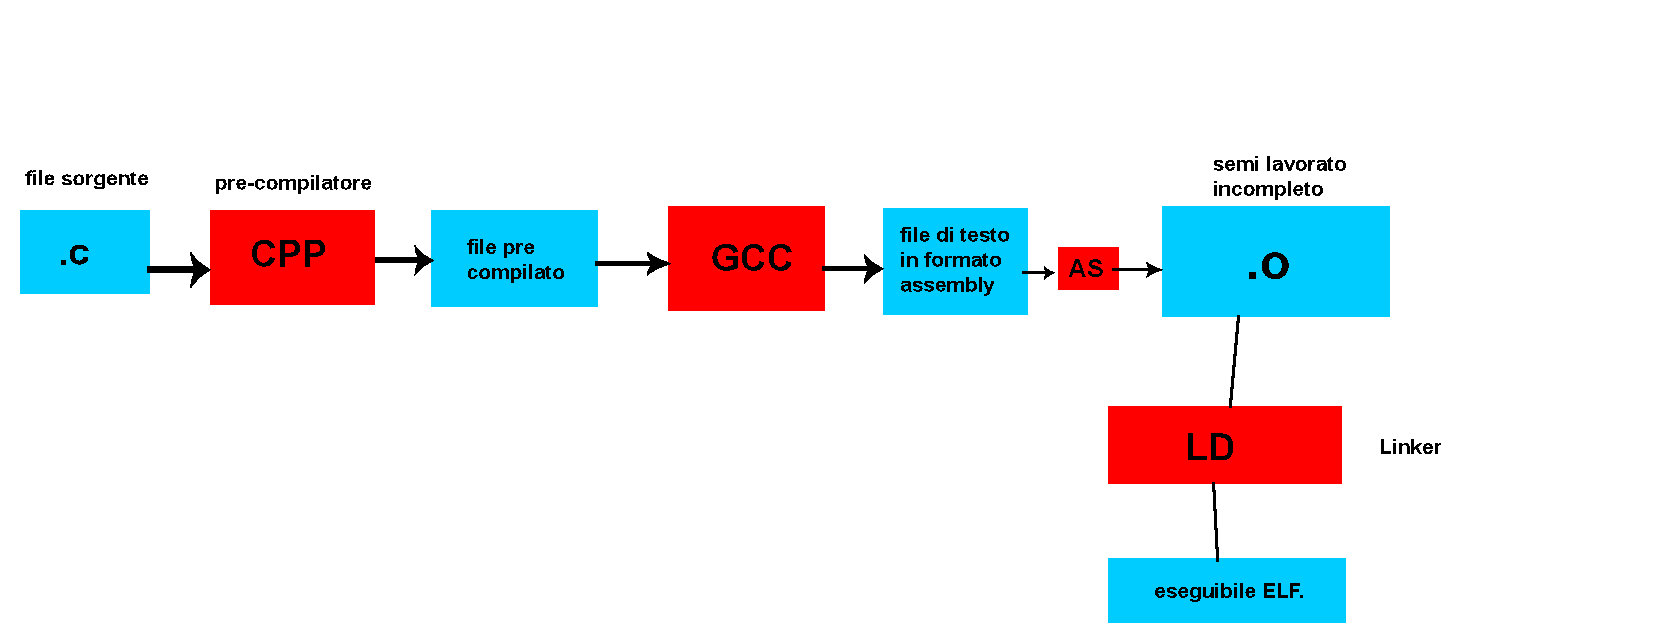
\includegraphics[width=15.5cm]{schema.pdf}
\label{fig:schema}
\end{figure}\\
Ovvero si parte dal .c, tramite un precompilatore si ottiene un file precompilato, dopodichè tramite gcc :\\
\begin{itemize}
\item Un assemblatore converte il file di testo in assembly generato da gcc in un .o
\item Un linker esegue il linking dinamico ottenendo un file in formato elf
\end{itemize}
Tipicamente i .o di sistema vengono inclusi in appositi raccoglitori con estensione .a, e vengono detti \textit{librerie}.\\
Il semilavorato non contiene il codice delle procedure invocate nel .c, e tiene una tabella di simboli che associa alcune funzioni utilizzate (o variabili) al programma .c\\
Il problema delle dipendenze è rappresentabile come un grafo e con questo nome si intende il problema per cui alcune librerie, per funzionare, hanno bisogno, a loro volta, di altre librerie.\\
\subsection{Direttive per il compilatore}
\begin{itemize}
\item \textbf{\#include} <nome\_libreria.h> oppure ''mia\_libreria.h'': Permette di includere una libreria nel file, in modo da poter sfruttare le funzioni dichiarate al suo interno. Con la include è come mettere il codice dei prototipi dentro il file che include la libreria. Ad esempio, se includo la stdio.h e uso la printf, è come se nel mio file avessi tutto il codice della printf all' interno.Dentro l'include troviamo:
\begin{itemize}
\item Prototipi
\item Definizioni di Simboli
\item Parte di compilazione condizionale
\end{itemize}
\item \textbf{\#ifdef} e \textbf{\#ifndef}: Due direttive che fanno parte della compilazione condizionale. In particolare ifdef è molto utile nello sviluppo di codice multipiattaforma:
\begin{lstlisting}
...
#ifdef __LINUX_H__
	//esegui codice linux.
	//Nota che il simbolo __LINUX_H__ e' di pura fantasia.
#else
	#ifdef __WINDOWS_H__
		//esegui codice windows.
		//Nota che il simbolo __WINDOWS_H__ e' di 
		//pura fantasia.
	#endif
#endif
...
\end{lstlisting}

\item \textbf{\#define}: Permette di definire simboli nel precompilatore accoppiati con una stringa:
\begin{lstlisting}
...
#define P 3.14
...
\end{lstlisting}
Come effetto ottengo che ogni volta uso P nel mio programma il compilatore lo sostituisce con 3.14.
\end{itemize}
\subsection{Compilazione condizionale}
La compilazione condizionale risulta molto utile in caso di /textit{multiple including}. Cosa si intende? Abbiamo visto come il problema delle dipendenze sia rappresentabile come un grafo; con questa idea in testa possiamo pensare ad una situazione come quella in figura, dove A e B sono due librerie scritte da due persone diverse: A conosce l'interfaccia che B ha dichiarato per la sua libreria.\\
\begin{figure}[h]
\centering
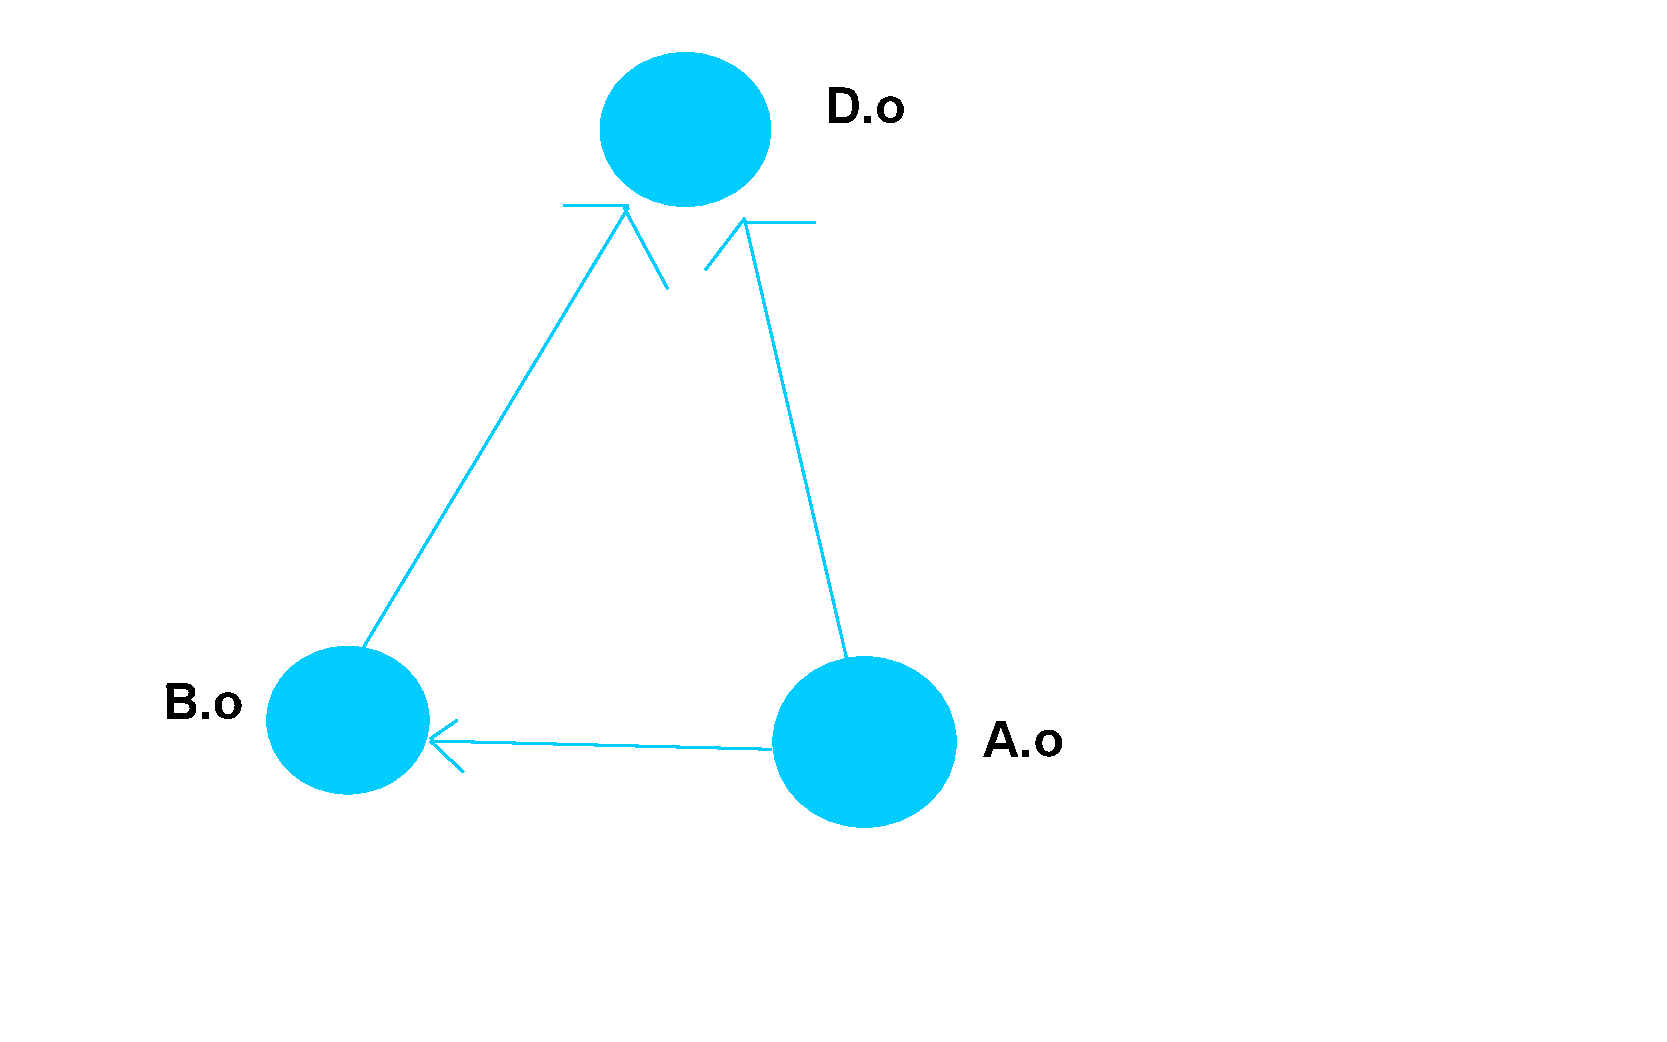
\includegraphics[width=15.5cm]{dipendenze.pdf}
\end{figure}\\
Il file A.c conterrà pertanto i seguenti include:
\begin{lstlisting}
...
#include <B.h>
#include <D.h>
...
\end{lstlisting}
Mentre il file B.c ...
\begin{lstlisting}
...
#include <D.h>
...
\end{lstlisting}
Guardando quel grafo possiamo notare come non sarebbe necessario includere anche D.h in A.c, poichè tale dichiarazione viene effettuata già da B.c: l'inclusione in A però rappresenta un \textbf{atto dovuto} perchè, se un domani il programmatore di B decidesse di cambiare il codice e non usasse più la libreria D.h, il programma smetterebbe di funzionare! Così però abbiamo sollevato un altro problema, allo stato attuale la libreria D.h è inclusa due volte! Per risolvere questo genere di situazioni entra in gioco la compilazione condizionale che funziona come segue:
\begin{lstlisting}
// fle D.h 
#ifndef __D_H__
	#def __D_H__
		...
		//codice di D.h
		...
	#endif
\end{lstlisting}
\textbf{E' in questo modo che vanno scritti correttamente gli include!}. In questo modo abbiamo ottenuto che, se quel simbolo non è definito allora viene definito e si include il codice, altrimenti nulla di fatto. Ciò si traduce con il fatto che una libreria può essere inclusa quante volte si vuole (anche IMPLICITAMENTE) e per il pre-compilatore conta come se fosse stata inclusa una volta sola!\\
Su linux la directory /usr/include contiene tutte le inclusioni.
\subsection{Linking Dinamico}
Il linking dinamico è un processo con cui il link sfrutta delle regioni di memoria condivisa per ridurre al minimo le dimensioni di un eseguibile. Ciò è possibile in virtù del fatto che le librerie dinamiche non vengono incluse nell' eseguibile ELF.
\subsection{Strumenti di Sistema}
\subsubsection{Gcc e le sue opzioni}
\begin{description}
\item -c ferma la compilazione al file oggetto
\item -S ferma la compilazione al codice assembly
\item -E ferma la compilazione al codice precompilato
\item -O genera codice ottimizzato
\item -Wall attiva tutti i warning
\item 
\item gcc hello.c -static -o hello : Non usa il linking dinamico
\end{description}
\subsubsection{Objdump, le sue opzioni, e altri programmi}
\begin{description}
\item objdump: Strumento che ci permette di eseguire il dump di un bin per debug/esplorazione. Le opzioni di objdump:
	\begin{description}
	\item -s : fa il dump di tutto.
	\item -T: esegue il dump e mostra la symbol table
	\item -D: disassembla il binario
	\end{description}
\item ldd nome\_file : mi dice con quali librerie è stato linkato il mio file
\item ltrace: Intercetta tutte le chiamate del programma alle librerie dinamiche
\end{description}

\section{Makefile}
Per i makefile si veda la cartella 09.
\section{It's time to debug}
\subsection{GDB - GNU DeBugger}
Il gdb è un potente debugger di binari in formato elf da linea di comando.\\
\textbf{Nota:} Per poter debuggare un programma bisogna compilarlo con l'opzione -g in modo da includere nel bin i simboli di debug.
\subsection{Avviare gdb}
Avviare gdb è molto semplice e si fa con il comando da shell:\\
\begin{center}
gdb <file\_da\_debuggare>
\end{center}
Fatto ciò ci troviamo difronte ad un prompt testuale:
\begin{lstlisting}

GNU gdb 6.3.50-20050815 (Apple version gdb-962) [...]
Copyright 2004 Free Software Foundation, Inc.
GDB is free software, covered by the GNU [...]
welcome to change it and/or distribute copies [...]
Type "show copying" to see the conditions.
There is absolutely no warranty for GDB.  Type [...]
This GDB was configured as "i386-apple-darwin"...
Reading symbols for shared libraries ... done

(gdb)_
\end{lstlisting}
A questo punto il programma aspetta da noi comandi.
\subsection{Il comando run}
Permette di lanciare un programma. Durante questa lezione useremo come studio di caso il seguente programma:
\begin{lstlisting}
1	#include <stdio.h>
2	
3	int main(){
4	    printf("hello World! \n");
5	    return 0;
6	}
\end{lstlisting}
Per lanciare la sua esecuzione usiamo il comando run.
\begin{center}
run prova.c
\end{center}
\textbf{Nota}: Il programma accetta per comodità anche solo la prima lettera del comando, in questo caso r, ma solo se non ci sono ambiguità tra due o più comandi.\\
In quel caso dobbiamo disambiguare il nome scrivendo più lettere:
\begin{lstlisting}
(gdb) run
Starting program: /Users/Alfredo/Uni/III ANNO/Algoritmi[...]
Reading symbols for shared libraries ++. done
hello World! 

Program exited normally.
\end{lstlisting}
\subsection{Il comando help}
Il comando help fornisce utili informazioni circa un particolare comando:
\begin{lstlisting}
(gdb) help run
Start debugged program.  You may specify arguments [...]
If 'start-with-shell' is set to 1, args may include [...]
they will be expanded using "sh".  Input and output [...]
">", "<", or ">>" will also be allowed.

With no arguments, uses arguments last specified [...]
To cancel previous arguments and run with [...]
use "set args" without arguments.
\end{lstlisting}
\subsection{Il comando list}
Fornisce il listato del programma, ma può essere impiegato come efficiente strumenti di ricerca di funzioni all' interno di un programma.
\textbf{Nota}: Dare due volte il comando list comporterà un errore da parte di gdb: questo è dovuto al fatto che il programma ha memoria \\
dei comandi dati e tenta di leggere oltre. Possiamo forzare il programma per leggere nuovamente il programma da capo scrivendo \textit{list 0}
\subsection{Il comando next}
Permette di avanzare nel programma ''entrando'' dentro un ciclo o una funzione.
\subsection{Il comando print}
Permette di stampare (solo una volta) il valore di una variabile:
\begin{lstlisting}
(gdb) print i
\end{lstlisting}
\subsection{Il comando display}
Permette di stampare, dopo ogni comandi impartito a gdb, il valore di una variabile:
\begin{lstlisting}
(gdb) display i
\end{lstlisting}
\subsection{Il comando step (into)}
Permette di avanzare nel programma ''entrando'' dentro un ciclo o una funzione.
\subsection{Il comando continue}
Prosegue con la normale esecuzione del programma senza fermarsi mai, a meno che non incontri un breakpoint.
\subsection{I breakpoint}
I breakpoint costituiscono gli strumenti più importanti per il debugging, in quanto permettono di fissare un punto all' interno del programma in
cui l'esecuzione dello stesso viene congelata, dandoci la possibilità di esplorare il mondo che ci circonda.
\subsubsection{Aggiungere un breakpoint}
 Inseriamo un breakpoint direttamente alla funzione principale:
\begin{lstlisting}
(gdb) break main
Breakpoint 1 at 0x1fd7: file prova.c, line 4.
\end{lstlisting}
Il debugger ci segnala che ha fatto quanto abbiamo richiesto.
\subsubsection{Disabilitare i breakpoint}
Ovviamente è possibile disabilitare temporaneamente un breakpoint nel caso non ci servisse più:
\begin{lstlisting}
(gdb) disable 1
\end{lstlisting}
Con questo comando abbiamo disabilitato il breakpoint appena creato.
\subsubsection{Eliminare un breakpoint}
Nel caso in cui ci accorgessimo che un breakpoint non sia più utile fino alla fine del debugging è sempre possibile eliminarlo:
\begin{lstlisting}
(gdb) delete 1
\end{lstlisting}
\subsubsection{I breakpoint condizionali}
GDB prevede la possibilità di inserire dei breakpoint condizionali, cioè attivabili solo al verificarsi di una determinata condizione:
\begin{center}
cond <numero\_del\_breakpoint> <condizione\_C-like>
\end{center}
\subsubsection{Ignorare i breakpoint}
Un' altra possibilità offerta da gdb è quella di ignorare i breakpoint per n volte, con n fissabile a piacere:
\begin{center}
cond <numero\_del\_breakpoint> <numero\_di\_volte\_che\_verrà\_ignorato>
\end{center}
Così scrivere una cosa del genere...
\begin{lstlisting}
(gdb) ignore 3 12
Will ignore next 12 crossings of breakpoint 3.
\end{lstlisting}
...produrrà come effetto che il breakpoint 3 verrà ignorato per 12 volte prima di diventare attivo.
\subsection{Esplorare lo stack}
E' possibile esplorare lo stack, andando a guardare il contenuto di ogni singolo frame allocato nello stack.
\subsubsection{Il comando bt}
Mostra lo stato corrente dello stack in un dato momento dell' esecuzione di un programma:
\begin{lstlisting}
(gdb) bt
#0  main () at prova.c:6
\end{lstlisting}
\subsubsection{Il comando up}
Permette (qualora ce ne fossero) di spostarsi nella pila, selezionando di volta in volta un frame allocato sempre più in alto.
\subsubsection{Il comando down}
Analogo ad up salvo per il fatto che in questo modo si scende verso il fondo della pila (verso il first in).
\subsubsection{Il comando info}
E' un utile comando che accetta diversi valori. \textit{info frame} fornisce informazioni sul frame corrente:
\begin{lstlisting}
(gdb) info frame
Stack level 0, frame at 0xbffff790:
 eip = 0x1fc4 in main (prova.c:6); saved eip 0x1f82
 source language c.
 Arglist at 0xbffff788, args: 
 Locals at 0xbffff788, Previous frame's sp is 0xbffff790
 Saved registers:
  ebx at 0xbffff784, ebp at 0xbffff788, eip at 0xbffff78c
\end{lstlisting}
Mentre \textit{info stack} fornisce la situazione dello stack:
\begin{lstlisting}
(gdb) info stack
#0  main () at prova.c:6
\end{lstlisting}

\section{Le utility diff e patch}
Queste due utility sono molto utili in grandi progetti quando si lavora in team; la prima mostra le differenze tra due file, creando una sorta di delta, la seconda applica il delta al primo file.
\subsection{diff}
Usage:\\
\begin{center}
\$ diff file1.txt file2.txt
\end{center}
\subsubsection{Opzioni di diff}
\begin{description}
\item -r data una directory genera le differenze ricorsivamente
\item -N elenca il contenuto dei file nuovi
\item -u elenca i file in formato unified
\end{description}
\subsection{patch}
Quello che fa patch si può riassumere così:
\begin{center}
patch = x1 + delta
\end{center}
dove delta = x2 - x1\\
\textbf{Nota}: Per essere indipendenti dalla directory in cui usiamo il comando usare l'opzione -p1.\\
Usage:\\
\begin{center}
patch [options] [originalfile [patchfile]]
\end{center}
cioè prende il delta (patchfile) e lo applica ad originalfile.
\subsection {Un esempio}
Create due cartelle:\\
proj1\\
----A.txt\\
proj2\\
----A1.txt\\

lanciamo i seguenti comandi:\\
\$ diff -ruN proj1/A.txt proj2/A2.txt > mypatch\\
e poi:\\
\$ patch -p1 -b proj1/A.txt mypatch\\

così abbiamo anche salvato il backup di A.txt
\end{document}